\documentclass{ctexrep}
\usepackage{CJK}
\usepackage{amsmath}
\CTEXsetup[format+={\flushleft}]{section}
\begin{document}
\title{单分类,在对抗样本缺失下的概念学习}
\author{David Martinus Johannes}
\date{January 25, 2015}
\maketitle
\chapter{导言}
如果让你在一个包含了苹果和梨的集合中区分这两类水果你会怎么做?这个问题看起来并不复杂,任何人都可以基于它们的长相或质感直接地区分它们。延伸开来,区分腐烂的或肮脏的两者,甚至是别的既非苹果也非梨的对象也不是一件困难的事。

尽管让人去区分苹果和梨并不困难,但让机器自动化这个过程却并不轻松。一个基本的问题:是什么让我们判定一个目标是‘苹果’,而另一个目标是‘梨’?是它们的质量、高度、颜色?还是说它们的形状、气味?最为可能的是,我们综合了上面的所有属性。现在暂且假定我们通过目标的颜色和气味来判定目标,那么,一个粘有泥土的苹果我们应给称它为什么?苹果?还是说泥土?

这就是我们所谓的分类问题:在一个事先已知的集合中(比如在这个案例中的苹果和梨)选取一个标签作为新目标的标签。分类器,基于一个样本集,对新目标执行分类操作(或者说对每一个输入对象赋予一个输出标签)。这篇文章并不关注与分类任务,我们关注的是另一个问题:单分类。在这个任务中,一个对象被判定为普遍的对象(比如苹果或梨)或异常的对象(其他类型的水果或者腐烂的水果或者外表肮脏的水果blabla)。

单分类问题与传统的分类问题有着本质的不同,在单分类问题中,我们夹着只有一个类别,即目标类别,的信息是可用的。这便意味着我们只能使用目标类别的样本作为训练集,而对其他类别的信息一无所知。我们需要在只掌握一个类别的信息下估计出两个类别的边界,这个任务实质上就是去定义出目标类别的边界,使得它尽可能多地接受目标对象的同时,尽可能地少地接受异常对象。

在第一章中,我们会给出整个研究的框架。由一个对统计模式识别的简单介绍开始,我们会提出一些经典的问题以及这些问题的一些可行解法,随后,我们引入文章的主题:单分类,并与传统的分类问题做对比。我们将看到,单分类问题会面临解决传统分类问题过程中遇到的问题,甚至更糟糕,因为单分类问题会引入一些额外的问题。

\section{从样本中学习}
在许多分类问题中,明确的规则并不存在(想想你能否明确地给出判定苹果和梨差异的规则),但样本却比较容易获取(比如找蔬菜水果商)。一个分类器,即一个接收输入对象并返回输出标签的函数,不可能通过已有的知识构建出来,因此,在模式识别或机器学习中,一种尝试是在(有限的)样本集中推理出一个分类器。训练样本的使用降低了人们对规则的需求,任务的目标变成寻找模型,并在训练集中学习规则,随后对对象进行预测。

‘对象’这个说法的含义非常泛,它涵盖了苹果、手写数字、语音信号、机器噪声等等。在本文中,我们假定用一个$d$维实数向量表示对象,所以一个对象$i$可以写为特征向量$x_i=(x_{i,1} \cdots x_{i, d})$,$x_{i, j} \in \mathcal{R}$(或简写为$x_i \in \mathcal{X}=\mathcal{R}^d$)。因此,一个对象就可以表示为特征空间$\mathcal{X}$中的一点。此外,我们假设向量中的每一个组成元素都是已知的,不存在缺失值。实际上,如果出于时间或金钱的考虑,为了得到较少的信息需要花费大量的金钱或时间,那么我们可能不对某些特征进行测量(这种情况在医学案例中尤为常见),此时就会出现特征缺失。特征缺失会引入额外的复杂性,我们并不打算考虑这种情况,我们只假定所有的特征都是可测量的。

我们还需要一个连续性假设,这在模式识别中是一个很普遍的假设:现实生活中,两个相似的对象在特征空间中位置相近。当我们处于特征空间中的一点,这个点代表了一个样本对象,如果我们稍微地改变它的位置,这个新位置所代表的对象应该与原位置代表的对象十分相似。这意味着我们假定对象并不是随机地而是像云团一样分散在特征空间中,从而一个对象的近邻代表了与他相似的另一个对象。如果没有这个连续性假设,我们不能期望从一小部分的样本中获取一个较好的分类器,因为决策边界可以在特征空间中随意放置,为了得到较好的分类效果将需要海量的样本。显然,为了区分对象,测量的特征需要蕴含足够的信息以区分它们,换言之,它们需要足够的表达能力,这样才能使得分类器拥有较好的泛化能力。如果我们只能测量到噪声,那么我们就别期望得到一个高性能的分类器了。

一个一般的多类分类器可以分解为多个两类分类器,因此,两类问题被认为是最基础的问题。在两类问题中,两个类别$\omega_1$和$\omega_1$被相应的标记为$-1$和$+1$。一个训练集包含了多个样本,每个样本$x_i$对应着一个标签$y_i$,$y_i \in \{-1, +1\}$:
\begin{equation}
\mathcal{X}^{tr} = \Big\{(x_i, y_i)|i=1, \cdots, N\Big\}
\end{equation}
对于分类器而言,需要从训练集中推理出一个函数$f(x)$,这个函数在给定输入$x$的时候给出一个输出标签$y = f(x)$:
\begin{equation}
f:\mathcal{R}^d \rightarrow \{-1, +1\}
\end{equation}

\begin{figure}[htbp]
  \centering
  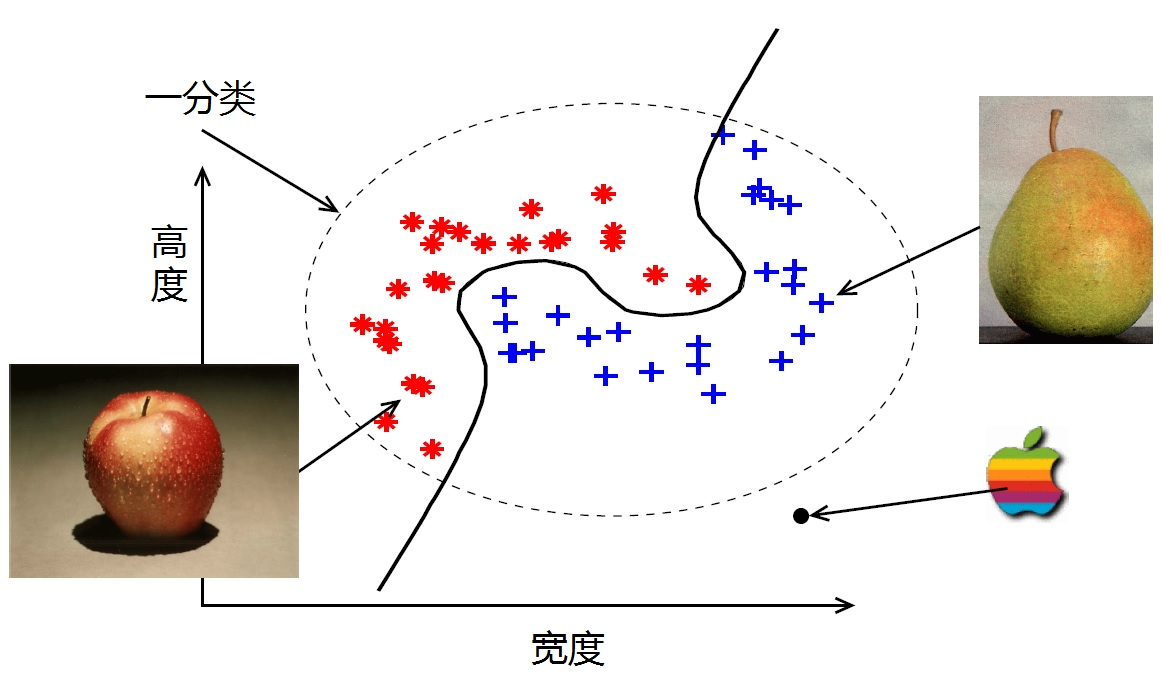
\includegraphics[width=0.9\textwidth]{figure/fig1.jpg}
  \caption{在一个包含了苹果和梨的训练集中应用传统分类与单分类,其中,每个对象包含两个特征。实线代表了传统分类器,用以区分苹果和梨,虚线描述了训练集。这个描述可以判定右下角的异常值(苹果商标),而在这个位置,传统的分类器会把它判定为梨}
  \label{fig:fig1}
\end{figure}

图\ref{fig:fig1}是本章开头引入的苹果-梨问题的数据集,每个对象有两个特征值(对象的宽度和高度,为了方便讨论,我们并没有引入额外的特征),因此每个对象$x$可以表示为一个2维特征空间中的一个点。图中,苹果用星号表示,梨用叉叉表示。原则上,对象可以散布在整个(2维)特征空间,但由于连续性假设,苹果与苹果,梨与梨之间相邻较近。另外,这两个测量值受到一些物理限制(宽度和高度不能为负,并且限制在某个值以下)

在苹果-梨的例子中,通过图\ref{fig:fig1}中的实线可以零错误地实现分类。但不幸的是,当引入右下角的异常苹果时,它会被判定为梨。在两类分类器的世界中,只有苹果和梨两个概念,所有的对象要么为苹果,要么为梨,不能为其他值,比如异常值。为了鉴定异常值,我们需要训练单分类器,单分类器的一个例子就是图\ref{fig:fig1}中的虚线。

\begin{figure}[htbp]
  \centering
  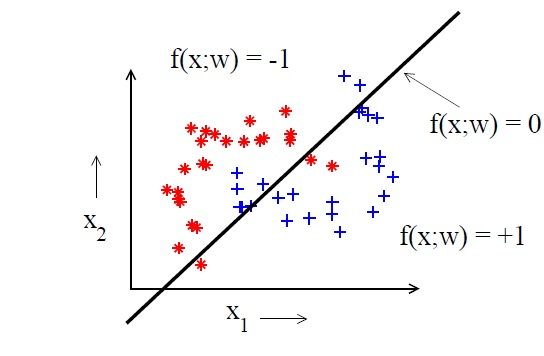
\includegraphics[width=0.9\textwidth]{figure/fig2.jpg}
  \caption{苹果-梨问题的一个解决方案。这里展示了一个简单的线性分类器$f(x;w)$,它观测每个对象的测量值$x_1$和$x_2$,并估计一个标签$f(x;w)=+1$或$f(x;w)=-1$。直线$f(x;w)=0$是线性决策面}
  \label{fig:fig2}
\end{figure}

大多数的函数$f$都是预先选好形式,只留下少量待确定的参数。函数可以记为$f(x;w)$来表明它依赖的参数,或者权值$w$(在下一章的特定例子中,参数被命名为$\alpha$)。这些函数具体的形式可能是线性函数、高斯混合模型、神经网络或者支撑向量机等。在图\ref{fig:fig2}中我们再次把苹果-梨问题搬出来讨论。这里,每个类别都有25个样本,图中的直线代表了一个线性分类器$f(x;w)$,尽管这并不是一个最有的线性分类器。对于大部分的对象,它正确地判定了其标签,但依然有7个梨和3个苹果被错误地判定。

为了在一个给定的训练集$\mathcal{X}^{tr}$中寻找的函数$f$的最优参数$w^*$,我们需要定义一个误差函数$\mathcal{E}(f, w, \mathcal{X}^{tr})$,由于我们假定训练集中大部分的对象都是独立同分布的,所以训练集上总的误差函数$f$可以分解为:
\begin{equation}
\mathcal{E}(f, w, \mathcal{X}^{tr}) = \frac{1}{N}\sum\limits_i \varepsilon\big(f(x_i; w), y_i\big)
\end{equation}
我们可以基于$f(x_i; w)$的不同形式定义不同的误差函数。对于离散的$f(x_i; w)$,误差函数可以定义为0--1损失,即被误分类的对象的总数:
\begin{equation}
\varepsilon_{0-1}\big(f(x_i;w), y_i\big) = \left\{
\begin{array}{cc}
0, & \text{若}f(x_i, w)=y_i,\\
1, & \text{其他}.
\end{array}
\right.
\end{equation}
例如,苹果-梨例子中,误差为$\mathcal{E}_{0-1}=10$。

对于实数函数$f(x_i; w)\in[-1,1]$而言,最常见的误差函数是均方误差(MSE):
\begin{equation}
\mathcal{E}_{\text{MSE}}\big(f(x_i;w)\big) = \big(f(x_i;w)-y_i\big)^2
\end{equation}
以及交叉熵,注意标签值需要为正数$y_i\in\{0,1\}$:
\begin{equation}
\mathcal{E}_{\text{ce}}\big(f(x_i;w)\big) = f(x_i;w)^{y_i}\big(1-f(x_i;w)\big)^{1-y_i}
\end{equation}

通过在训练集中最小化误差$\mathcal{E}$,有可能找到一个较好的权值$w$,从而得到一个高性能的分类器。

\end{document}